\section{Results}
\label{sec:results}
\subsection{Method comparison}
Table~\ref{tbl:cmu_method_comparison} shows the results comparing the different methods on the CMU Kids data both for simulated and real errors.
AUC values are reported together with 95\% confidence intervals computed according to~\cite{HanleyAndMcNeil1982ROC-CI}.
The methods based on models trained with CTC outperform both methods based on models trained with CE (GOP-DNN-Avg and GOP-CE-Avg).
%GOP-CE-Avg outperforms GOP-DNN-Avg
GOP-CTC-SF-S, that is, the segmentation-free method restricted to substitution errors is significantly better on the simulated errors whereas GOP-CTC-SF-SD, that also allows deletion errors is significantly better on the real errors.
This can be explained by the fact that simulated errors are produced exclusively by substitution, but real errors may include deletions as well.
The standard evaluation criterion used here only considers phones in the canonical transcription.
This means that insertion errors only have an effect on the evaluation if they modify the pronunciation of the neighbouring canonical phones.
This does not allow to show the full potential of GOP-CTC-SF-SDI, that in our tests performs worse than GOP-CTC-SF-SD.
However, defining an ad-hoc evaluation criterion is outside the scope of this study.
%shows ) does not seem to help for this dataset.
%This may be due to the evaluation method that only considers phonemes in the canonical transcription.
%For these results it seems that insertion errors are not common in the test data.

\begin{table*}
\centering
\caption{Phone Recognition and Pronunciation Assessment Results vs Peakiness.
%The models are selected on the certain updating steps that has the minimum validation loss during training
}
\label{table:results_vs_peakiness}
% \input{tabels/results_vs_peakiness}
\begin{tabular}{ l|ccc|ccc }
% \hline
% \multicolumn{5}{c}{The overview of the models} \\
 \hline\hline
  & \multicolumn{3}{c|}{Peakiness and Phone Recognition} & \multicolumn{3}{c}{GOP Methods (AUC, 95\% confidence intervals)} \\
 Models & BC (\%) & ConEn & PER (\%) & GOP-X-Avg & GOP-X-SA & GOP-X-SF \\
 \hline
CE         & 42.22 & 22.9886 & 13.25 & 0.860 ($\pm$2.91E-3)~\cite{cao24b_interspeech} & 0.885 ($\pm$2.50E-3) & 0.870 ($\pm$2.75E-3) \\
EnCTC-0.20 & 79.10 & 37.8672 & 11.63 & 0.842 ($\pm$3.19E-3) & 0.860 ($\pm$2.91E-3) & 0.913 ($\pm$2.01E-3) \\
EnCTC-0.15 & 79.55 & 35.9145 & 11.64 & 0.841 ($\pm$3.20E-3) & 0.861 ($\pm$2.81E-3) & \textbf{0.915 ($\pm$1.97E-3)} \\
EnCTC-0.10 & 80.11 & 34.9024 & 11.47 & 0.841 ($\pm$3.20E-3) & 0.864 ($\pm$2.84E-3) &  \textbf{0.914 ($\pm$1.99E-3)} \\
EsCTC      & 88.52 & 14.2370 & 21.06 & 0.580 ($\pm$6.00E-3) & 0.884 ($\pm$2.52E-3) & 0.896 ($\pm$2.31E-3) \\
CTC        & 88.62 & 2.8287  & 11.46 & 0.824 ($\pm$3.46E-3) & 0.909 ($\pm$2.08E-3) &  \textbf{0.914 ($\pm$1.99E-3)} \\
 \hline\hline
\end{tabular}

\end{table*}

\subsection{Performance versus peakiness}
Table~\ref{table:results_vs_peakiness} shows the results of testing the effect of peakiness of the acoustic models on the real errors of the CMU Kids.
All the models were trained up to checkpoint 8000.
The left part of the table reports blank coverage (BC) as a measure of POT and conditional entropy (ConEn) as a measure of POS, as well as phone error rates.
The right part of the table reports MDD results.
The models were ordered in the table in increasing order of peakiness over time (POT).

Standard CTC results in the highest BC and lowest ConEn, which means that CTC is the peakiest model both with respect to POT and POS. 
It is also the best phone recognizer with the lowest PER among the models.

For the EnCTC models, POS decreases as the weight $\beta$ of the entropy term in the loss function increases.
In our tests we varied $\beta$ in the range $[0.10,0.15,0.20]$.
This is not surprising because the entropy term is similar to ConEn.
More interesting is the fact that POT also decreases with $\beta$ as shown by BC.
The EnCTC performance in phone recognition seems to degrade with the peakiness of the models.

The model trained with EsCTC has the highest PER, a similar POT compared to CTC but a much lower POS (higher ConEn).
This is in line with the experiments in~\cite{CTC-ME}, because the model makes the strong assumption that the labels should be uniformly distributed over time which is not always true for speech. 
%As a result, the peaky activations of EsCTC often fall out of the area of the baseline alignment. 

As we expected, the model trained with CE has the lowest BC because it is trained frame-wise according to baseline segmentation.
Surprisingly, the ConEn of the CE-trained model is still lower than EnCTC implying that the distribution of possible alignment paths are more concentrated for CE-trained model. 

%\subsection{MDD results}

%\begin{table}
%\centering
%\caption{AUC values for CMU Kids, both simulated error and real error}
%\label{table:cmu}
%\input{tabels/cmu_auc_vs_peakiness}
%\end{table}

The experimental results for MDD are shown in the right side of Table~\ref{table:results_vs_peakiness} in terms of AUC and 95\% confidence intervals.
When using the standard GOP definition (GOP-X-Avg), the CE model performs the best.
This is expected because GOP-X-Avg uses the same baseline segmentation that was used to train the CE model.
The CTC and EnCTC models are comparable.
We believe that this is because, although the models have different degrees of peakiness, their activation is still within the segments defined by the baseline segmentation.
On the contrary, the AUC of GOP-EsCTC-Avg is particularly low, most probably because the model activations do not necessarily follow standard speech segmentation.
It is therefore possible that GOP is evaluated, in this case, based on activations other than the target phoneme.
This interpretation is also supported by the fact that the use of the self-aligned definition (GOP-EsCTC-SA) gives results that are comparable with the model trained with CE.
However, GOP-X-Avg is clearly outperformed by the proposed GOP-X-SA and GOP-X-SF methods that will be analyzed next.

In general, the proposed GOP-X-SA is always superior to GOP-X-Avg, suggesting that this method is able to focus on the regions corresponding to the relevant model activations.
%Moving on to the column of GOP-X-Align.
%We can see from the table that the performance of this method is generally better than GOP-X-avg, regardless of the model being used.
It is interesting to note that this phenomenon can be observed even for the models trained with CE, for which the mismatch between model activations and baseline segmentation should be minimal.
%Even for CE, whose model's activation is the closest to the baseline-alignment, it is still $3\%$ relatively better with GOP-X-Align than with GOP-X-Avg.
%It convinces us that the segmentation used for phoneme-level MDD with traditional GOP should focus on the place of activation rather than the acoustic evidence.
%In other words, for using traditional GOP with Eq.\eqref{eqa:gop-dnn}, it is suggested to re-align after training of a phoneme recognizer. 
Among the different models, CTC training performs the best when using GOP-X-SA.
% Our interpretation is that CTC results in a more discriminative model than CE as verified by the PER.
% Our self-aligned definition of GOP (GOP-X-SA) makes it possible to take advantage of this more performant model if compared to the standard definition (GOP-X-Avg).
Our interpretation is that the  self-aligned definition of GOP (GOP-X-SA) prefers to work with peaky models~(both POT and POS) such as the model trained with CTC. 
Comparing to the standard definition (GOP-X-Avg), this method makes it possible to take advantage of the highly-discriminative model which is often good for recognition.
%Notably, there is a drop of performance when switched from CTC model to CE model. 
%It can be explained by our hypothesis in Sec.\ref{sec:gop-ctc-align} that the separation brought by CTC's POT is beneficial to alignment errors, since those two models have the biggest gap of BC shown in table.~\ref{table:cmu}.
% This interpretation is also supported by the slight degradation in AUC results for the EnCTC models, that mimics the same degradation in phone recognition results.
This interpretation is also supported by the slight degradation in AUC results compared to standard CTC for the EnCTC models which are less peaky and less performant in terms of PER.
%Also we can see from the results that the EnCTC models perform worse than CTC model, and the AUC drops further when coping with EnCTC trained with higher entropy weights $\beta$.  
%This can also explained by the drop of BC, but more significantly is the increasing of ConEn.
% An exception to this interpretation is, however, the behavior of the model trained with EsCTC which has by far the worse phone recognition performance, but has a very similar performance to CE when using GOP-X-SA.
Exceptionally, the behavior of the model trained with EsCTC has by far the worst phone recognition performance.
However, the model's peakiness~(with the second highest BC and second lowest ConEn) could still make it comparable with CE in MDD performance when combined with GOP-X-SA.
%As discussed in Sec.\ref{sec:gop-ctc-af}, the method GOP-X-Align still relies on one single alignment that might lose some information of many other competitive paths due to uncertainty of the alignment.
%Interestingly, even though EsCTC is the worst phoneme recognizer~(in terms of PER) and its activation disregard the acoustic evidence badly, it works almost as good as CE in MDD task with GOP-X-Align which is much better than EnCTC. 
%This can be also explained by the high level of BC~(indicating high degree of separation of information) and relative low value of ConEn~(indicating not many alternative alignments exist).

Finally, the last column of the table reports the results with the proposed segmentation-free method (GOP-X-SF).
This method obtains the best overall performance for MDD by a significant margin.
Furthermore, according to the confidence intervals it is not possible to determine which acoustic model performs the best with this method because the results obtained with CTC and EnCTC are not statistically different.
This is in accordance with our hypothesis that GOP-X-SF would be less affected by POS of the acoustic models, compared to methods that rely on segmentation.
%, we are happy to see that the AUC of EnCTC models are back to the level of CTC after that the method GOP-X-AF tries to collect the information for MDD from all the alternative alignments. 
%Therefore the hypothesis that GOP-X-AF is robust to POS or alignment error is empirically proved and the best performance of this work is obtained with the combination GOP-EnCTC-0.15-AF.
%Actually, general improvements of performance are observed when compared GOP-X-AF to GOP-X-Align except for CE-trained model.
%We suspect that is due to the difference of interpretation between CTC's blank tokens and CE's SIL tokens during ASR training.
%However in our experiments of GOP-CE-AF, we treat them equally and implement the method by simply replacing blank with SIL. 
%Here we can make two observations: the first is that the alignment-free method is less affected by peakiness than the other two methods we have tested.
We can also observe that, by considering all possible segmentations, GOP-X-SF is able to extract much more useful information for MDD not only compared to the external segmentation (GOP-X-Avg) but also compared to an alignment that is matched to the activations of the acoustic model (GOP-X-SA).

\begin{figure*}
    \centering
    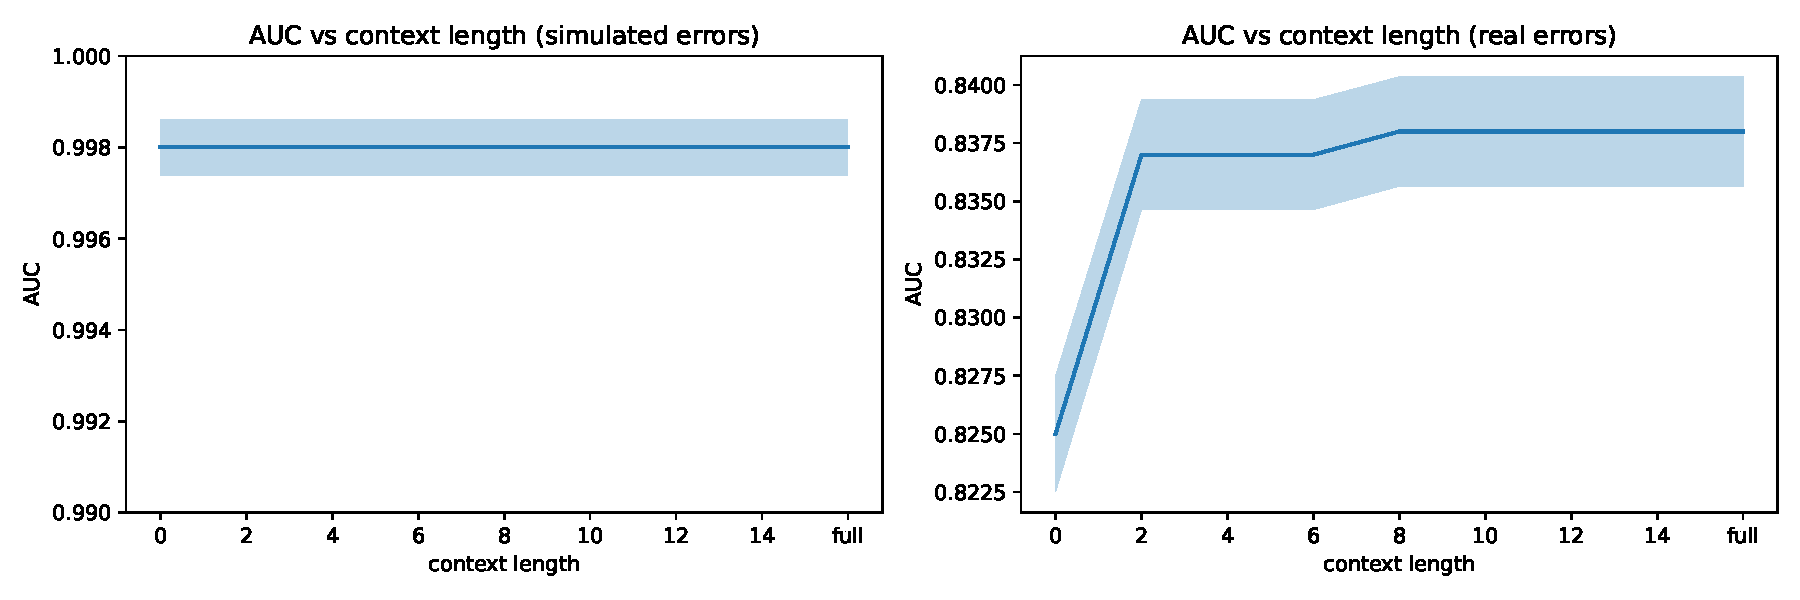
\includegraphics[width=\textwidth]{figs/auc_vs_context_subplots.pdf}
    \caption{AUC versus context length for simulated and real errors on the CMU Kids data.
    The shaded area shows 95\% confidence intervals computed with \cite{HanleyAndMcNeil1982ROC-CI}.}
    \label{fig:auc_vs_context}
\end{figure*}

%\begin{table}
%\centering
%\caption{AUC for CMU Kids, tested with different number of phonemes as context}
%\input{tabels/context_exp}
%\label{table:context-len-exps}
%\end{table}



\subsection{GOP-SF and context length}
By definition, the segmentation-free GOP method that we have proposed (GOP-SF) is computed considering contributions from the entire utterance, even if those contributions are weighted by how likely it is that each part of the utterance belongs to the target phone.
%on each utterance individually, but the GOP values need to be comparable across utterances for MDD.
A reasonable question to ask is how the length of left context~(\Lleft) and right context~(\Lright) affect the pronunciation assessment results.

Figure~\ref{fig:auc_vs_context} displays the AUC results on CMU Kids where we have varied the number of phones in \Lleft and \Lright from 0 to 7 resulting in a total context length from 0 to 14 in increments of 2.
We also report results with the original utterances (full context).
In this case, the length of the context depends on the specific utterance, but it is always greater than~14.
The left plots simulated errors, whereas the right plots real errors.
%We first selected as target intermediate phones with more than 7 phones left and right in the transcription.
%We then used self-alignment to crop the model's activations to match the context length condition under test.
%Finally, we calculated AUC based on GOP-CTC-AF on the cropped activations.

For simulated errors, the AUC values for different context lengths remain at a high level, and the impact of context length can be neglected.
%Due to the fact that simulated errors are synthesized for correct utterances only and there is only one possible substitution error at a time~(by flipping the phoneme at the target position) in the utterance, the self-alignment can be relatively accurate.
The results show that GOP-CTC-SF is robust to different context length in the ideal case. 
 
Also for real errors, the dependency on context length is usually under the variability described by the 95\% confidence intervals.
The only exception is when we reduce the context to zero, which corresponds to the self-aligned GOP definition (GOP-SA).
This confirms the superiority of the segmentation-free method that is able to take advantage of the context to assess the pronunciation of the target phoneme.
Using context lengths between 8 and 14 is visually indistinguishable from using the full context length.
This suggests that the information needed to assess the pronunciation of the target phoneme is relatively local in the utterance.
%On the other hand, for real errors, the AUC is lower with the reduced context, especially around length 0 to 2.
%The AUC then increases together with the incremental of context length and reaches the same level at 8 as with the full context.
%Unlike the case of simulated single substitution error, in reality, one utterance can have multiple errors in the context as well, which violates the implicit assumption when we made the graph in Fig.\ref{fig:af-gragh}. 
%As a result, the cropped activations may not correctly match the left- and right-context. 
%It means that by looking at Eq.\ref{eq:gop-sf_forward}, the $\alpha$ term and the $\beta$ term can be evaluated incorrectly.
%For shorter context length, e.g, 1-2, the consequence can be very significant.
%However, the bias and variance of GOP-CTC-AF could be eliminated with context length longer than 6, as the proposed method GOP-AF becomes more robust and performant when takes longer observations and larger context length into account in real cases.

%Noting that for context length equals to 0, due to POS of CTC, the GOP-AF method is reduced to GOP-SA. 
%The degradation can be mostly likely attributed to the wrongly cropped activation. 
%We can re-emphasis from here the importance of getting rid of forced alignment for GOP because of the existence of alignment issues and/or the pronunciation errors other than substitutions. 
%The experiment is designed as follows: 
%we start from the single middle phoneme~($\text{context-len}=0$) in \Lcano of an utterance and for each time $t>=1$ adding two surrounding context($\text{context-len}=2t$).  
%Instead of selecting the speech signal for the modified phonemes labels using baseline-alignment, we run Viterbi on post-softmax activations of the last layer of the neural network~(The CTC head), similarly to GOP-X-Align. 
%With the alignment, we are able to select the parts of the activations for the corresponding phonemes together with the shortened canonical sequence for computing GOP-CTC-AF as usual. 
%We compute GOP-CTC-AF on the middle phoneme of the utterances from CMU Kids that have no errors and their middle phonemes have has at least $14(\pm7)$ context length.
%For those phonemes we also synthesize substitution errors for comparison as done by~\cite{cao23_interspeech}.
%The Fig.\ref{fig:context-len} shows us that the GOP-CTC-AF is quite invariant over different context length.
%It means the GOP generated by this method can be used for MDD on utterances with different length of canonical phoneme sequences.
%It also tells that the variation brought by context length is small enough compared to the distance of mean between correct and incorrect phonemes~(synthesized substitution).
% \begin{figure}[t]
%   \centering
%   \includegraphics[width=1\columnwidth]{figs/std.png} 
%       \caption{The mean and standard deviation of the method GOP-CTC-SF of correct phoneme and synthesized substitution errors, from context length 0 to full canonical sequence.}
%   \label{fig:context-len}
% \end{figure}

\begin{table}
\centering
\caption{speechocean762, reported with Pearson correlation coefficients}
\label{table:so}
% \input{tabels/speechocean_table}
\begin{tabular}{ lcc  }
 \hline\hline
% \multicolumn{3}{|c|}{Speechocean762} \\
% \hline
 Features & MDD model & PCC \\
 \hline
 GOP-TDNN~\cite{cao24b_interspeech} & poly. reg. &0.361$\pm$0.008 \\
 GOP-CE-SF-SD & poly. reg. & N/A\\
GOP-CE-SF-SD-\textit{numerical}&poly. reg. & 0.314$\pm$0.008 \\
GOP-CE-SF-SD-Norm& poly. reg. & 0.332$\pm$0.008 \\
GOP-CTC-SF-SD~\cite{cao24b_interspeech}& poly. reg. & 0.433$\pm$0.007 \\
GOP-CTC-SF-SD-\textit{numerical}&poly. reg. & \textbf{0.450}$\pm$\textbf{0.006} \\
GOP-CTC-SF-SD-Norm& poly. reg. & \textbf{0.449}$\pm$\textbf{0.006} \\
 \hline
 FGOP-TDNN~\cite{speechocean762}& SVR &0.441$\pm$0.007 \\
 FGOP-CTC-SF~\cite{cao24b_interspeech}& SVR &0.568$\pm$0.006 \\
FGOP-CTC-SF-\textit{numerical}&SVR&\textbf{0.580$\pm$0.006} \\
FGOP-CTC-SF-Norm&SVR&\textbf{0.581$\pm$0.006} \\
 \hline
  FGOP-TDNN~\cite{GOPT} & GOPT & 0.605$\pm$0.002 \\
  FGOP-CTC-SF~\cite{cao24b_interspeech} & GOPT & 0.618$\pm$0.002 \\
  FGOP-CTC-SF-\textit{numerical} & GOPT & \textbf{0.646}$\pm$\textbf{0.002} \\
  FGOP-CTC-SF-Norm & GOPT & \textbf{0.648}$\pm$\textbf{0.002} \\
  %FGOP-CTC-SF-Norm-child & GOPT & \textbf{0.635}$\pm$\textbf{0.005} \\
  %FGOP-CTC-SF-Norm-adult & GOPT & \textbf{0.651}$\pm$\textbf{0.004} \\
     \hline\hline
\end{tabular}

\end{table}

\subsection{Comparison to state-of-the-art}
In order to compare the performance of our best method~(GOP-X-SF-SD) with respect to the state-of-the-art, we report results on the speechocean762 dataset in Table~\ref{table:so}.
The table compares different scalar definitions of GOP with a simple polynomial regression MDD model.
It also includes results with GOP feature vectors in combination with SVR or GOPT MDD models.

Similarly to the previous experiments on CMU Kids, we find that the methods relying on models trained with the CE loss are less performant than those trained with the CTC loss. 
Results for the method ``GOP-CE-SF-SD'' are missing due to numerical problems.
%, some GOP values in the utterances with multiple pronunciation errors become infinity because of the numerical issues caused by too many mismatches of the activations with the canonical.~(It is not that apparent for CTC-trained models due to the reason of many blank tokens).
These were solved in the new implementation (``GOP-CE-SF-SD-\textit{numerical}'').
The results are further improved using the definition that normalizes GOP by the estimated length of the target segment (``GOP-CE-SF-SD-Norm'').

In all cases, when combined with a CTC-trained model, our segmentation-free methods (GOP-CTC-SF, and FGOP-CTC-SF) outperform the baseline methods that use traditional GOP with the Time-Delayed-Neural-Network~(TDNN) acoustic models by a significant margin.
We also see improvements when using the implementation which solves the numerical issues compared to our previous results. 
As we expected, the extra normalization steps for the methods are less significant for CTC-trained acoustic models than CE-trained ones. 
The best combination of our method is ``FGOP-CTC-SF-Norm'' which has  $5.01\%$ relatively higher PCC than previously reported. 
We also tested this method on the split of the speechocean762 test set that separates children~(age $\leq 11$) from adults~(age $> 11$).
The corresponding PCCs are $0.635\pm 0.005$ (children) and $0.651\pm 0.004$ (adults).
The slight gap between child and adult result may be reduced by adapting the acoustic models to child speech.

At the time of writing and to the best of our knowledge, the highest phoneme-level PCC obtained for the speechocean762  dataset is $0.693$~\cite{chao23_interspeech}.
The relatively limited PCC improvements of this model with respect to ours are, however, obtained at the cost of higher computational complexity, heavier feature engineering and more sophisticated loss functions that take all the linguistic aspects into account.
For this reason, we believe that our method is still preferable for practical real-world applications.

Finally, we could not find results on pure end-to-end models for MDD on the speechocean762 data.
This is probably due to the limited amount of training data which prevents the proper training of those models.
